% Copyright 2026 Sreeram Anil
% SPDX-License-Identifier: CC-BY-4.0
% =============================================================================
%  OCV inversion (voltage lookup) — baseline family
% =============================================================================
\chapter{Open-Circuit-Voltage Inversion (OCV Lookup)}
\label{ch:ocvlookup}

\section*{At a glance}
\begin{tabular}{@{}l>{\raggedright\arraybackslash}p{0.76\textwidth}@{}}
Family & baselines \\
Header & \texttt{include/estkit/battery/baselines.hpp} \\
Registered name & \texttt{OCVLookup} \\
State dimension & $n_x = 4$; $\soc$ replaced each step, $v_1,v_2,h$ propagate open-loop \\
Cost per step & $\mathcal{O}(n_b)$ with $n_b=40$ bisection steps, $\approx 1310$\,ns/step, no heap \\
Primary references & \cite{plett2015bms1,weng2014ocv,hu2012comparative} \\
\end{tabular}

\section{Motivation and relevance}
Coulomb counting integrates and therefore drifts; the natural complement is a method with no memory
at all --- invert the cell's equilibrium characteristic and read the state of charge off the
terminal voltage. The two fail in exactly opposite ways, and it is the pairing that motivates every
model-based filter in this report: a Kalman filter is precisely a rule for weighting a drift-free
but noisy voltage inversion against a smooth but drifting ampere-hour integral, with the weight
computed from the two error covariances.

The difficulty is that the open-circuit voltage is not measurable in flight. The terminal voltage
during a \SI{22.5}{\ampere} hover differs from the OCV by more than \SI{0.4}{\volt}, against an OCV
span of \SI{1.3}{\volt} over the whole SOC range, so a voltage-lookup method is really a model-based
\emph{overpotential-compensation} method and its numbers are best read as a measurement of the
ECM's fidelity. Its relevant property for an aircraft is the one Coulomb counting lacks: bounded
error. After a reset, a lost non-volatile store or a mid-flight power cycle, the estimate returns to
within the model error in a time set by one filter constant --- a certification-friendly property,
and the reason it survives in production systems as a re-initialisation path.

\section{Problem statement}
The measurement model of Chapter~\ref{ch:ecm} is
\begin{equation}
v \;=\; \ocv(\soc,T) \;+\; M h \;-\; v_1 \;-\; v_2 \;-\; R_0(T)\,i ,
\label{eq:ocv-meas}
\end{equation}
with $v_1,v_2$ the RC overpotentials, $h\in[-1,1]$ the hysteresis state and $M$ its magnitude.
\begin{assumption}\label{as:ocv-all}
(i) $\ocv(\cdot,T)$ is strictly monotone in $\soc$, so $\ocv^{-1}$ exists; (ii) $R_0(T)$, $R_j$,
$\tau_j$, $M$ are known and $v_1,v_2,h$ can be reconstructed from the current history alone;
(iii) $\soc$ varies slowly compared with the low-pass constant $\tau_{\text{lp}}$.
\end{assumption}
Item~(i) holds for this cell but only just --- the slope falls to \SI{0.197}{\volt} near
$\soc=0.90$. Item~(ii) is what \code{param\_mismatch}, \code{cold} and \code{preisach} test; item
(iii) is what fails during the hovers.

\section{Derivation}
Rearranging \eqref{eq:ocv-meas} for the compensated open-circuit voltage,
\begin{equation}
\widehat{\ocv}_k \;=\; v^{\text{m}}_k + R_0(T^{\text{m}}_k)\, i^{\text{m}}_k
 + \hat v_{1,k} + \hat v_{2,k} - M\,\hat h_k ,
\label{eq:ocv-compensate}
\end{equation}
where $\hat v_1,\hat v_2,\hat h$ come from propagating the model's $f$ open-loop with the measured
current --- the same recursion Coulomb counting uses, but here only the overpotential states are
kept and $\soc$ is overwritten each step. The instantaneous SOC is
$\hat\soc^{\text{inst}}_k = \ocv^{-1}(\widehat{\ocv}_k, T^{\text{m}}_k)$, computed by 40 bisection
steps on $[-0.05,1.05]$ against the 241-point table, which resolves the interval to
$1.1/2^{40}\approx10^{-12}$. Bisection rather than Newton is used because it needs no derivative,
cannot diverge, and has a data-independent trip count (\S\ref{sec:lib-mcu}).

This inherits the full voltage noise amplified by the inverse slope, so a first-order low-pass with
$\tau_{\text{lp}} = \SI{30}{\second}$ is applied:
\begin{equation}
\hat\soc_k \;=\; a\,\hat\soc_{k-1} + (1-a)\,\hat\soc^{\text{inst}}_k,
\qquad a = e^{-\dt/\tau_{\text{lp}}} = 0.99667 .
\label{eq:ocv-lowpass}
\end{equation}
Its noise rejection is $\sqrt{\dt/(2\tau_{\text{lp}})} = 0.041$ in standard deviation: a
\SI{2}{\milli\volt} voltage noise over a \SI{0.8}{\volt} slope is \SI{0.25}{\percent} of SOC per
sample, filtered to \SI{0.010}{\percent}. That is the noise floor; everything else is bias.

Linearising the inversion about the true SOC, the estimate error is the compensated-voltage error
divided by the OCV slope:
\begin{equation}
\boxed{\;
\hat\soc^{\text{inst}} - \soc \;=\;
\frac{\delta v + \delta R_0\, i + \delta v_1 + \delta v_2 - M\,\delta h}{\partial\ocv/\partial\soc}
\;+\;\mathcal{O}\!\left(\tfrac{\partial^2\ocv}{\partial\soc^2}\right) \; }
\label{eq:ocv-error}
\end{equation}
Three consequences dominate the benchmark.

\emph{The slope is the gain, and it collapses on the plateau.} For this NMC811/graphite cell
$\partial\ocv/\partial\soc$ is \SIrange{0.71}{1.16}{\volt} over most of $[0.2,0.85]$, so a
\SI{10}{\milli\volt} model error costs about \SI{1.2}{\percent} of SOC; but between $\soc=0.86$ and
$0.93$ the two-phase behaviour of the graphite electrode flattens the curve to \SI{0.197}{\volt} at
$\soc\approx0.895$, where the same error costs \SI{5.1}{\percent}. Every mission starts at
$\soc_0=0.95$ and falls through this plateau in its first minutes.

\emph{The low-pass converts a rate into a bias.} Applying \eqref{eq:ocv-lowpass} to a truth ramping
at $\dot\soc$ gives a steady-state lag
\begin{equation}
\hat\soc - \soc \;\longrightarrow\; -\tau_{\text{lp}}\,\dot\soc \;=\; +\,\frac{\tau_{\text{lp}}\,i}{3600\,Q},
\label{eq:ocv-lag}
\end{equation}
positive on discharge --- the estimate is stale and therefore too high. At the eVTOL cruise
($i=\SI{5.5}{\ampere}$) this is \SI{0.92}{\percent}; during the \SI{22.5}{\ampere} hover,
\SI{3.75}{\percent}. This single term explains the shape of the nominal error trace and is the
method's central tension: $\tau_{\text{lp}}$ must be large to reject noise through a slope gain of
$1/0.2$ to $1/1.2$, and small to avoid lag, and no value is good at both. A filter that weights the
two information sources by their covariances is not a refinement of this method --- it is the
resolution of this dilemma.

\emph{Model error enters multiplied by the current.} $\delta R_0\,i$ is \SI{22.5}{\milli\volt} for a
\SI{1}{\milli\ohm} resistance error at hover, i.e.\ \SI{2.8}{\percent} of SOC at a \SI{0.8}{\volt}
slope; at \SI{-10}{\celsius}, where $R_0$ is \SI{35.1}{\milli\ohm}, the same \emph{relative} error
costs three times as much.

\section{Algorithm}
\begin{algorithm}[H]
\caption{OCV inversion with IR/RC compensation --- one sampling period}
\begin{algorithmic}[1]
\Require $\hat\soc_{k-1}$, overpotential states $\hat v_{1},\hat v_{2},\hat h$, stored $\vu_{k-1}$, new $i^{\text{m}}_k, v^{\text{m}}_k, T^{\text{m}}_k$
\State $\vu_k \gets [\,i^{\text{m}}_k,\ T^{\text{m}}_k\,]^\T$
\If{$k>0$} \State $\xhat \gets f(\xhat,\vu_{k-1})$ \Comment{open-loop RC and hysteresis states}
\EndIf
\State $\hat v_k \gets h(\xhat,\vu_k)$ \Comment{diagnostic voltage prediction}
\State $\widehat{\ocv} \gets v^{\text{m}}_k + R_0(T^{\text{m}}_k)\,i^{\text{m}}_k + \hat v_1 + \hat v_2 - M\hat h$
\State $\hat\soc^{\text{inst}} \gets$ \textbf{bisect} $\ocv(\cdot,T^{\text{m}}_k) = \widehat{\ocv}$ on $[-0.05,1.05]$, 40 steps
\State $\hat\soc_k \gets a\,\hat\soc_{k-1} + (1-a)\,\hat\soc^{\text{inst}}$
\State $\xhat[\soc] \gets \hat\soc_k$; \quad $\vu_{k-1}\gets\vu_k$
\Ensure $\hat\soc_k$
\end{algorithmic}
\end{algorithm}
Line~8 writes the filtered SOC back into the model state, which acts only through the
current-dependence of the hysteresis rate and is second order.

\section{Application and implementation notes}
$\tau_{\text{lp}} = \SI{30}{\second}$ is the only tuning constant, fixed for all scenarios. The
bisection bracket matches the model's \code{constrain} bounds, so the estimate is clamped to the
physical range without a separate projection, and the estimator uses \code{EstimatorConfig::params}
for $R_0(T),R_1,\tau_1,R_2,\tau_2,M$ --- exactly what \code{param\_mismatch} perturbs --- with the
measured temperature for the Arrhenius and entropic terms.

Cost is dominated by the 40 bisection steps: \SI{1310}{\nano\second}, sixteen times Coulomb counting
and $2.7\times$ the EKF. That ranking is worth pausing on --- the ``simple'' baseline is the
expensive one --- and it is entirely an artefact of solving a scalar equation by bisection rather
than by two Newton steps from the previous estimate, which would cost about \SI{80}{\nano\second}.
\code{sizeof} is \SI{4192}{\byte}, essentially all OCV table, which here is genuinely needed. There
is no covariance to lose definiteness; the float32 build matches the double build to within
\SI{0.01}{\percent} of SOC, the bisection simply ceasing to improve after about step 24 --- an
argument for reducing the trip count on a 32-bit target.

\section{Benchmark results}
% Copyright 2026 Sreeram Anil
% SPDX-License-Identifier: CC-BY-4.0
\begin{table}[H]\centering\footnotesize\setlength{\tabcolsep}{4pt}
\caption{OCVLookup: cell-level benchmark on the eVTOL mission (mean over seeds; RMSE and max error in \% SOC; $t_\mathrm{conv}$: first time the error stays below 2\,\% for 60\,s, -- = never; EKF reference: steady-state RMSE of the plain EKF on the same data).}\label{tab:cell_OCVLookup}
\begin{tabular}{llrrrrrcrr}\toprule
plant & scenario & RMSE & RMSE$_\mathrm{ss}$ & max & $t_\mathrm{conv}$ [s] & RMSE$_v$ [mV] & div. & EKF ref. & ns/step \\ \midrule
ECM & nominal & 1.53 & 1.30 & 4.30 & 0 & 11.74 & no & 0.05 & 1310 \\
ECM & init\_error & 3.32 & 1.30 & 34.88 & 77 & 23.45 & no & 0.05 & 1312 \\
ECM & current\_bias & 2.48 & 2.13 & 7.62 & 0 & 11.94 & no & 0.61 & 1310 \\
ECM & noise\_step & 1.53 & 1.31 & 4.30 & 0 & 11.72 & no & 0.12 & 1307 \\
ECM & outliers & 1.53 & 1.31 & 4.29 & 0 & 11.83 & no & 0.21 & 1305 \\
ECM & cold & 1.82 & 1.56 & 5.38 & 0 & 11.90 & no & 0.16 & 1308 \\
ECM & hot & 1.45 & 1.24 & 3.96 & 0 & 11.76 & no & 0.03 & 1312 \\
ECM & aged\_cell & 1.86 & 1.38 & 6.94 & 0 & 21.76 & no & 1.52 & 1306 \\
ECM & param\_mismatch & 0.90 & 0.41 & 4.22 & 0 & 13.63 & no & 1.36 & 1310 \\
ECM & sensor\_dropout & 1.58 & 1.30 & 4.79 & 0 & 11.82 & no & 0.46 & 1307 \\
ECM & preisach & 1.82 & 2.15 & 4.90 & 0 & 11.33 & no & 0.20 & 1308 \\
ECM & combined & 2.64 & 1.15 & 24.91 & 66 & 22.18 & no & 12.44 & 1305 \\
\midrule
SPM & nominal & 1.77 & 2.03 & 5.79 & 0 & 12.55 & no & 3.73 & 1310 \\
SPM & init\_error & 3.50 & 2.03 & 34.88 & 87 & 23.32 & no & 3.81 & 1294 \\
SPM & current\_bias & 2.21 & 2.49 & 6.70 & 0 & 12.64 & no & 5.69 & 1309 \\
SPM & noise\_step & 1.77 & 2.03 & 5.79 & 0 & 12.53 & no & 3.30 & 1295 \\
SPM & outliers & 1.77 & 2.03 & 5.67 & 0 & 12.61 & no & 1.99 & 1270 \\
SPM & cold & 4.85 & 6.11 & 15.29 & 306 & 19.78 & no & 7.35 & 1295 \\
SPM & hot & 2.06 & 1.98 & 6.96 & 0 & 12.14 & no & 2.16 & 1300 \\
SPM & param\_mismatch & 1.25 & 0.60 & 3.60 & 0 & 12.69 & no & 3.13 & 1292 \\
SPM & sensor\_dropout & 1.80 & 2.03 & 6.40 & 0 & 12.66 & no & 5.31 & 1307 \\
\bottomrule\end{tabular}\end{table}

\begin{figure}[H]\centering
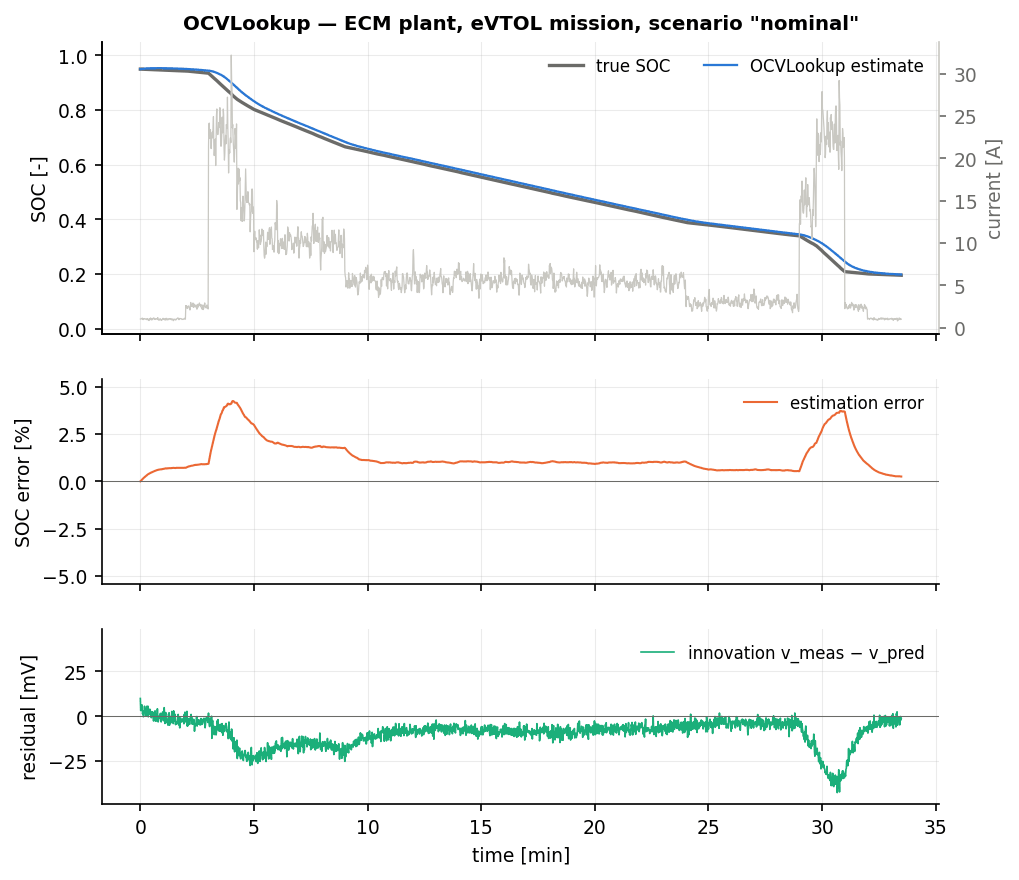
\includegraphics[width=0.78\textwidth]{figures/cell_OCVLookup_nominal.png}
\caption{OCV inversion on the nominal eVTOL mission. The error trace is the low-pass lag
\eqref{eq:ocv-lag}: about $+1\,\%$ through the cruise, rising to $+4\,\%$ during each hover and
decaying with the \SI{30}{\second} filter constant. The residual panel shows the
$-\SI{25}{\milli\volt}$ hover excursions that \eqref{eq:ocv-compensate} fails to remove.}
\end{figure}
\begin{figure}[H]\centering
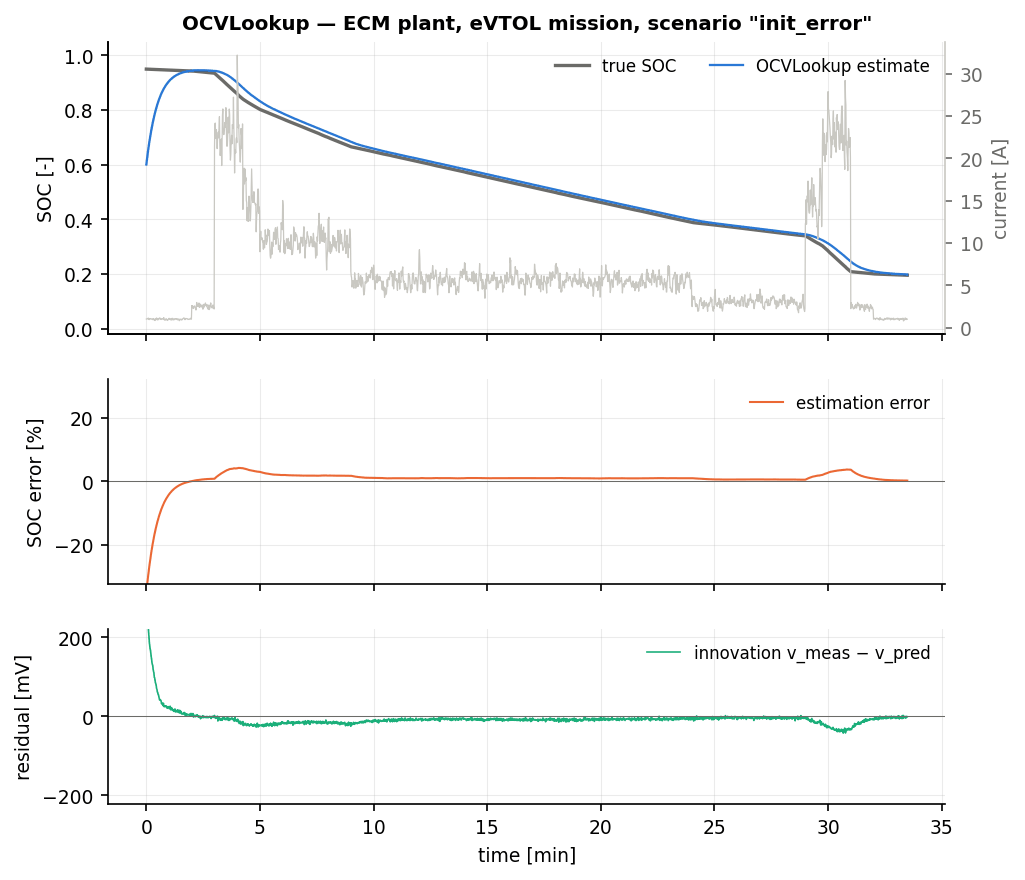
\includegraphics[width=0.78\textwidth]{figures/cell_OCVLookup_init_error.png}
\caption{OCV inversion with a $-35\,\%$ initial SOC error: removed exponentially with the
\SI{30}{\second} constant, after which the trace is indistinguishable from the nominal one. Compare
Chapter~\ref{ch:coulombcounting}, where the same error persists for the whole mission.}
\end{figure}

The headline numbers invert those of Coulomb counting in every respect. On the nominal eVTOL mission
$\text{RMSE}_{\text{ss}} = 1.30\,\%$, nearly four times Coulomb counting's $0.36\,\%$ and
twenty-six times the EKF's $0.05\,\%$; but on \code{init\_error} the steady-state figure is
\emph{also} $1.30\,\%$, with $t_{\text{conv}} = \SI{77}{\second}$ and no divergence, against Coulomb
counting's $35.35\,\%$ and a divergence flag. The method has no memory, so it has no way to be wrong
about the past, and the recovery time predicted by \eqref{eq:ocv-lowpass},
$\tau_{\text{lp}}\ln(0.35/0.02) = \SI{86}{\second}$, brackets the measured value.

The $\text{RMSE}_v$ column sits at \SI{11.7}{\milli\volt} in almost every scenario, against Coulomb
counting's \SI{3.4}{\milli\volt} and the EKF's \SI{0.79}{\milli\volt}. This looks paradoxical for a
method that fits the voltage, and it is the clearest illustration in the report of what
$\text{RMSE}_v$ measures: the method does \emph{not} fit the voltage, it inverts each sample
independently and then filters the result, so the reported state lags and the voltage recomputed
from that lagged state is correspondingly wrong. Fitting and filtering are different operations, and
the EKF is the one that does both at once.

Three scenarios repay a closer look. \code{param\_mismatch} is the method's best column at
$0.41\,\%$ --- three times better than its own nominal result and than the EKF's $1.36\,\%$ --- and
this is a coincidence that should be reported as one: at the cruise current of \SI{5.5}{\ampere},
$R_0\times0.7$ under-compensates the ohmic drop by \SI{19.8}{\milli\volt} while $R_1\times1.3$
over-compensates the fast branch by \SI{9.9}{\milli\volt}, a net $-\SI{9.9}{\milli\volt}$ in
$\widehat{\ocv}$, i.e.\ $-1.2\,\%$ of SOC, which nearly cancels the $+0.9\,\%$ lag of
\eqref{eq:ocv-lag}. Move to a different current and the cancellation disappears.

\code{preisach} is the worst ECM column at $2.15\,\%$ steady-state (whole-run $1.82\,\%$, peak
$4.90\,\%$): the plant's 32-relay operator has a major-loop half-width of \SI{15}{\milli\volt}, with
the charging branch above the discharging branch, against the estimator's $M=\SI{5}{\milli\volt}$,
so $-M\hat h$ removes at most a third of the true hysteresis and does so with the wrong path
dependence. Fifteen to twenty millivolts of uncompensated hysteresis is
\SIrange{1.9}{2.5}{\percent} of SOC at mid-slope, which is the steady-state figure; the peak occurs
on the plateau. Note that the hysteresis is the one term of \eqref{eq:ocv-error} that does not
shrink with current, so it is also what limits the load-gated hybrid of
Chapter~\ref{ch:coulombocvhybrid} ($2.28\,\%$), while Coulomb counting --- which ignores the voltage
--- is unaffected at $0.36\,\%$.

\paragraph{The SPM plant.} On the electrochemical plant the estimators use a 2-RC circuit fitted to
the single-particle model with a \SI{4}{\milli\volt} structured residual (Chapter~\ref{ch:spm}), and
because \eqref{eq:ocv-error} divides the compensation error by the OCV slope, that residual lands
directly on the estimate: $\text{RMSE}_{\text{ss}} = 2.03\,\%$ on \code{nominal} against
$1.30\,\%$ on the ECM plant, and $2.03\,\%$ again on \code{noise\_step}, \code{outliers} and
\code{sensor\_dropout}, since none of those touch the compensation. The degradation is modest
because a \SI{4}{\milli\volt} structural residual is of the same order as the lag term that already
dominates the ECM result. \code{cold} is the outright failure: $6.11\,\%$ steady-state,
$15.29\,\%$ peak, $t_{\text{conv}} = \SI{306}{\second}$, against Coulomb counting's $0.47\,\%$ on
the same data. At \SI{-10}{\celsius} the single-particle model's solid-diffusion overpotential is
large, strongly SOC-dependent and not representable by a constant-parameter 2-RC circuit, so
\eqref{eq:ocv-compensate} is wrong by tens of millivolts and \eqref{eq:ocv-error} converts that
straight into SOC error. When the voltage model breaks down, using the voltage is worse than
ignoring it. The one SPM row that improves on the ECM plant is \code{param\_mismatch} at
$0.60\,\%$ --- the same accidental cancellation as before, now working against a different residual.
Against the EKF the comparison is favourable on \code{nominal} ($2.03\,\%$ versus $3.73\,\%$) and
unfavourable on \code{cold} ($6.11\,\%$ versus $7.35\,\%$ --- both bad), which places OCV inversion
and the EKF in the same band on this plant for the first time: both are limited by the same
measurement model.

\section{Summary}
Use OCV inversion when the estimate must be bounded regardless of history: after a reset, as a
re-initialisation path, as an independent monitor of a drifting primary estimator, or on a duty
cycle with long rests where \eqref{eq:ocv-compensate} reduces to $\widehat{\ocv}\approx v$. Do not
use it as the primary in-flight estimator of a high-power aircraft --- the lag \eqref{eq:ocv-lag} is
\SI{3.75}{\percent} of SOC at hover and cannot be tuned away, the plateau at $\soc\approx0.9$
multiplies every model error by five, and it is more expensive than the EKF that dominates it in ten
of twelve scenarios. Its real contribution is diagnostic: read alongside Coulomb counting it
decomposes the problem into a drift term and a model term, and every filter in Parts~III--X is a
particular compromise between them.
